\chapter{Ants}
\label{sec:module.Ants}


\section{State-Klassen}
\label{sec:module.Ants.State}

\begin{figure}[H]
\centering
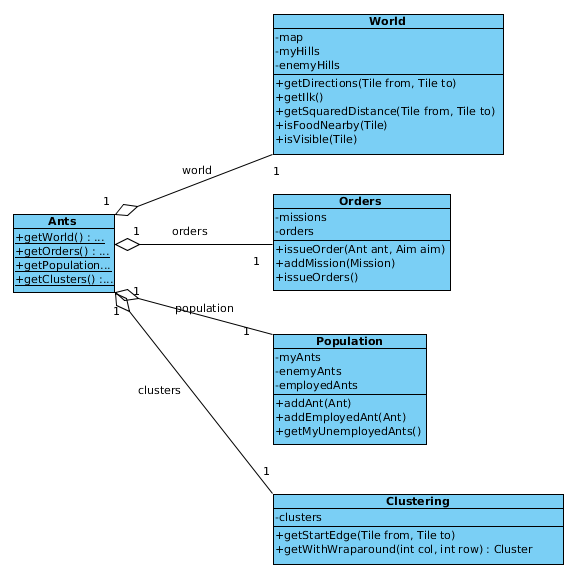
\includegraphics[width=0.7\textwidth]{91_bilder/State}
\caption{State-Klassen (vereinfacht)}
\label{fig:StateClasses}
\end{figure}

Abbildung \ref{fig:StateClasses} zeigt eine \"{U}bersicht �ber die Zustands-Klassen. F�r das Diagramm wurden lediglich die wichtigsten Methoden und Attribute ber�cksichtigt. Die State-Klassen implementieren alle das Singleton-Pattern.

\subsection{Ants}
\label{sec:module.Ants.State.Ants}
Die Ants Klasse ist die zentrale State-Klasse. Sie bietet auch einfachen Zugriff auf die anderen State-Klassen. Urspr�nglich hatten wir alle Methoden, die mit dem Zugriff auf den Spielzustand zu tun hatten, direkt in der Ants Klasse implementiert, haben aber schnell gemerkt, dass das unhandlich wird. Die Ants Klasse dient jetzt vor allem als Container f�r die anderen State-Klassen und implementiert nur noch einige Methoden, die Zustands�nderungen in verschiedenen Bereichen vornehmen.

\subsection{World}
\label{sec:module.Ants.State.World}
Die World Klasse enth�lt Informationen zur Spielwelt. Hier wird die Karte abgespeichert, in der f�r jede Zelle die aktuell bekannten Informationen festgehalten werden. Das beinhaltet die Sichtbarkeit der Zelle und was die Zelle aktuell enth�lt (Ameise, Nahrung, Wasser, ...). Ausserdem werden Listen gef�hrt, wo sich die eigenen und die bekannten gegnerischen H�gel befinden. Die Klasse bietet Methoden zur Distanzberechnung, gibt Auskunft �ber einzelne Zellen und dar�ber, ob sich Nahrung in der Umgebung einer bestimmten Zelle befindet.

\subsection{Orders}
\label{sec:module.Ants.State.Orders}
In der Orders Klasse wird �ber Befehle und Missionen der einzelnen Ameisen Buch gef�hrt. Die Liste der Befehle wird dabei in jedem Zug geleert und neu bef�llt, w�hrend die Liste der Missionen zug�bergreifend gef�hrt wird. Das zentrale Verwalten der Befehle und Missionen dient dazu, sicherzustellen, dass keine widerspr�chlichen Befehle ausgegeben werden wie: mehrere Befehle f�r eine Ameise, gleiche Ziel-Koordinaten f�r mehrere Ameisen, eine Ameise in mehreren Missionen etc.

\subsection{Population}
\label{sec:module.Ants.State.Population}
Die Population Klasse dient der Verwaltung der eigenen und der gegnerischen Ameisen-V�lker. Hier werden die Ameisen mit ihren aktuellen Aufenthaltsorten festgehalten. Wenn f�r eine Ameise ein Befehl ausgegeben wird, wird die Ameise als besch�ftigt markiert. \"{U}ber die Methode \texttt{getMyUnemployedAnts()} kann jederzeit eine Liste der Ameisen abgefragt werden, die f�r den aktuellen Zug noch keine Befehle erhalten haben.

\subsection{Clustering}
\label{sec:module.Ants.State.Clustering}
Die Clustering Klasse dient dem Aufteilen des Spielfeldes in Clusters f�r die HPA*-Suche (s. Abschnitt \ref{subsec:module.Suchalgorithmen.Pfadsuche.HPAstar}). Hier werden die berechneten Clusters abgelegt, damit diese nicht bei jeder Verwendung neu berechnet werden m�ssen. Der Zugriff auf sie erfolgt ebenfalls �ber die Clustering Klasse.

\section{Spiel-Elemente (Ants-Spezifisch)}
\label{sec:module.Ants.State.Entities.Ants}

\begin{figure}[H]
\centering
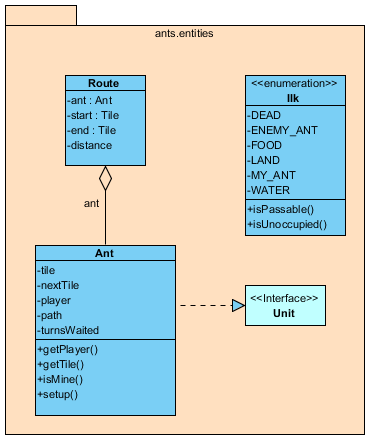
\includegraphics[width=0.5\textwidth]{91_bilder/antsEntities}
\caption{Ants-spezifische Elemente der Spielwelt (vereinfacht)}
\label{fig:antsEntities}
\end{figure}

TODO NEW IMAGE (Searchtarget)

Abbildung \ref{fig:antsEntities} zeigt die wichtigsten Klassen, die die Elemente des Spiels repr�sentieren. Der \"Ubersichtlichkeit wegen wurden nur die wichtigsten Attribute und Operationen in das Diagramm aufgenommen.

\subsection{Ant}
\label{sec:implementation.Entities.Ant}
Eine Ant geh�rt immer zu einem Spieler; �ber die Methode isMine() k�nnen unsere eigenen Ameisen identifiziert werden. 
Eine Ameise weiss jeweils in welcher Zelle sie steht. Das Feld nextTile dient der Verfolgung einer Ameise �ber mehrere Z�ge -- das Feld wird jeweils aktualisiert, wenn der Ameise ein Befehl ausgegeben wird. Im n�chsten Zug k�nnen wir dann pr�fen ob die Ameise den Befehl korrekt ausf�hren konnte. Eine Ameise kennt auch die anderen Ameisen in ihrer Umgebung: �ber die Methoden getEnemies()/FriendsInRadius() k�nnen alle bekannten Freunde und Feinde in einem bestimmten Radius ermittelt werden.


\subsection{Route}
\label{sec:implementation.Entities.Route}
Eine Route repr�sentiert eine einfache Start-Ziel Verbindung. Sie h�lt f�r eine Ameise die Luftliniendistanz zu einem bestimmten Zielfeld fest.

\subsection{Ilk}
\label{sec:implementation.Entities.Ilk}
Ilk ist der Typ einer Zelle. Der Ilk einer Tile-Instanz gibt an, was sich gerade in der Zelle befindet. Dies kann ein Gel�nde-Typ sein, wenn die Zelle ansonsten leer ist, oder es kann eine Ameise, Nahrung, oder ein H�gel sein. Die Ilk-Enumeration bietet Hilfsmethoden, um festzustellen, ob eine Zelle passierbar oder besetzt ist.

\section{Spiel-Elemente (Ants-Spezifisch)}
\label{sec:module.Ants.State.Entities.Ants}

\begin{figure}[H]
\centering
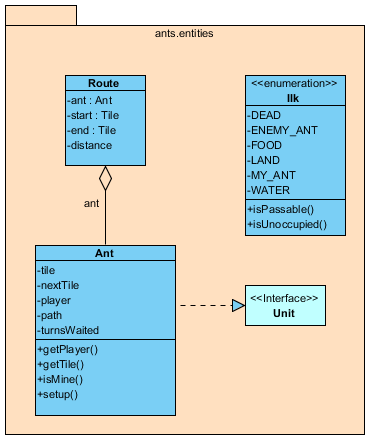
\includegraphics[width=0.5\textwidth]{91_bilder/antsEntities}
\caption{Ants-spezifische Elemente der Spielwelt (vereinfacht)}
\label{fig:antsEntities}
\end{figure}
